\documentclass[journal,12pt,twocolumn]{IEEEtran}
 \usepackage{setspace}
 \usepackage{gensymb}
 \usepackage{graphicx}
 \singlespacing
\graphicspath{ {/user/adarshsrivastava/desktop/Matrix Theory/Assignemnt_5} }
 \usepackage[cmex10]{amsmath}
 \usepackage{amsthm}
 \usepackage{hyperref}
 \usepackage{mathrsfs}
 \usepackage{txfonts}
 \usepackage{stfloats}
 \usepackage{bm}
 \usepackage{cite}
 \usepackage{cases}
 \usepackage{subfig}
 \usepackage{longtable}
 \usepackage{multirow}
 \usepackage{enumitem}
 \usepackage{mathtools}
 \usepackage{steinmetz}
 \usepackage{tikz}
 \usepackage{circuitikz}
 \usepackage{verbatim}
 \usepackage{tfrupee}
 \usepackage[breaklinks=true]{hyperref}
 \usepackage{tkz-euclide}
 \usetikzlibrary{calc,math}
 \usepackage{listings}
     \usepackage{color}                                            %%
     \usepackage{array}                                            %%
     \usepackage{longtable}                                        %%
     \usepackage{calc}                                             %%
     \usepackage{multirow}                                         %%
     \usepackage{hhline}                                           %%
     \usepackage{ifthen}                                           %%
     \usepackage{lscape}     
 \usepackage{multicol}
 \usepackage{chngcntr}
 \DeclareMathOperator*{\Res}{Res}
 \renewcommand\thesection{\arabic{section}}
 \renewcommand\thesubsection{\thesection.\arabic{subsection}}
 \renewcommand\thesubsubsection{\thesubsection.\arabic{subsubsection}}
 \renewcommand\thesectiondis{\arabic{section}}
 \renewcommand\thesubsectiondis{\thesectiondis.\arabic{subsection}}
 \renewcommand\thesubsubsectiondis{\thesubsectiondis.\arabic{subsubsection}}
 \hyphenation{op-tical net-works semi-conduc-tor}
 \def\inputGnumericTable{}                                 %%
 \lstset{
 %language=C,
 frame=single, 
 breaklines=true,
 columns=fullflexible
 }
 \begin{document}
 \newtheorem{theorem}{Theorem}[section]
 \newtheorem{problem}{Problem}
 \newtheorem{proposition}{Proposition}[section]
 \newtheorem{lemma}{Lemma}[section]
 \newtheorem{corollary}[theorem]{Corollary}
 \newtheorem{example}{Example}[section]
 \newtheorem{definition}[problem]{Definition}
 \newcommand{\BEQA}{\begin{eqnarray}}
 \newcommand{\EEQA}{\end{eqnarray}}
 \newcommand{\define}{\stackrel{\triangle}{=}}
 \bibliographystyle{IEEEtran}
 \providecommand{\mbf}{\mathbf}
 \providecommand{\pr}[1]{\ensuremath{\Pr\left(#1\right)}}
 \providecommand{\qfunc}[1]{\ensuremath{Q\left(#1\right)}}
 \providecommand{\sbrak}[1]{\ensuremath{{}\left[#1\right]}}
 \providecommand{\lsbrak}[1]{\ensuremath{{}\left[#1\right.}}
 \providecommand{\rsbrak}[1]{\ensuremath{{}\left.#1\right]}}
 \providecommand{\brak}[1]{\ensuremath{\left(#1\right)}}
 \providecommand{\lbrak}[1]{\ensuremath{\left(#1\right.}}
 \providecommand{\rbrak}[1]{\ensuremath{\left.#1\right)}}
 \providecommand{\cbrak}[1]{\ensuremath{\left\{#1\right\}}}
 \providecommand{\lcbrak}[1]{\ensuremath{\left\{#1\right.}}
 \providecommand{\rcbrak}[1]{\ensuremath{\left.#1\right\}}}
 \theoremstyle{remark}
 \newtheorem{rem}{Remark}
 \newcommand{\sgn}{\mathop{\mathrm{sgn}}}
 \providecommand{\abs}[1]{\left\vert#1\right\vert}
 \providecommand{\res}[1]{\Res\displaylimits_{#1}} 
 \providecommand{\norm}[1]{\left\lVert#1\right\rVert}
 %\providecommand{\norm}[1]{\lVert#1\rVert}
 \providecommand{\mtx}[1]{\mathbf{#1}}
 \providecommand{\mean}[1]{E\left[ #1 \right]}
 \providecommand{\fourier}{\overset{\mathcal{F}}{ \rightleftharpoons}}
 %\providecommand{\hilbert}{\overset{\mathcal{H}}{ \rightleftharpoons}}
 \providecommand{\system}{\overset{\mathcal{H}}{ \longleftrightarrow}}
 	%\newcommand{\solution}[2]{\textbf{Solution:}{#1}}
 \newcommand{\solution}{\noindent \textbf{Solution: }}
 \newcommand{\cosec}{\,\text{cosec}\,}
 \providecommand{\dec}[2]{\ensuremath{\overset{#1}{\underset{#2}{\gtrless}}}}
 \newcommand{\myvec}[1]{\ensuremath{\begin{pmatrix}#1\end{pmatrix}}}
 \newcommand{\mydet}[1]{\ensuremath{\begin{vmatrix}#1\end{vmatrix}}}
 \numberwithin{equation}{subsection}
 \makeatletter
 \@addtoreset{figure}{problem}
 \makeatother
 \let\StandardTheFigure\thefigure
 \let\vec\mathbf
 \renewcommand{\thefigure}{\theproblem}
 \def\putbox#1#2#3{\makebox[0in][l]{\makebox[#1][l]{}\raisebox{\baselineskip}[0in][0in]{\raisebox{#2}[0in][0in]{#3}}}}
      \def\rightbox#1{\makebox[0in][r]{#1}}
      \def\centbox#1{\makebox[0in]{#1}}
      \def\topbox#1{\raisebox{-\baselineskip}[0in][0in]{#1}}
      \def\midbox#1{\raisebox{-0.5\baselineskip}[0in][0in]{#1}}
 \vspace{3cm}
 \title{Assignment 5}
 \author{Adarsh Srivastava}
 \maketitle
 \newpage
 \bigskip
 %\renewcommand{\thefigure}{\theenumi}
 \renewcommand{\thetable}{\theenumi}
 The link to the solution is
 \begin{lstlisting}
  https://github.com/Adarsh1310/EE5609
 \end{lstlisting}
 \begin{abstract}
 This documents solves a problem based on circles.
 \end{abstract}
  \section{\textbf{Problem}}
 Find the area of the region bounded by the circle $\bf{x}^{T}$ $\bf{x}$= 4 and \norm{\vec{x}-\myvec{2\\0}}=2.
  \section{\textbf{Solution}}
  \norm{\vec{x}}^2 + 2\vec{u}^T\vec{x} + f = 0\\
  {\vec{x}^T\vec{x}} + 2\vec{u}^T\vec{x} + f = 0\\
  $So from above equation we can say that,
  \subsection{Circle 1}
  Taking equation of the first circle to be,
 \begin{align}
 \norm{\vec{x}}^2 + 2\vec{u}_1^T\vec{x} + f_1 = 0\label{2.1.1}\\
 {\vec{x}^{T}\vec{x}}-4=0 \label{2.1.2}\text{(given)}\\
 \vec{u_1}=\myvec{0\\0}\\
 f_1=-4\\
\vec{O_1}=\myvec{0\\0}
 \end{align}
 
 \subsection{Circle 2}
Taking equation of the second circle to be,
\begin{align}
  \norm{\vec{x}-\myvec{2\\0}}^2=2^2 \text{(given)}\\
  {\vec{x}^{T}\vec{x}+2\vec{u_2}^T\vec{x}}=0 \label{2.2.2}\\
  \vec{u_2}=\myvec{-2\\0}\\
 f_2=0\\
 \vec{O_2}=\myvec{2\\0}
  \end{align}
 Now,Subtracting equation \eqref{2.2.2} from \eqref{2.1.2} We get,
 \begin{align}
 \vec{x}^T\vec{x}-2\vec{u_2}^T\vec{x}+f_1-\vec{x}^{T}\vec{x}=0\\
 2\vec{u}^{T}\vec{x}=-4\\
 \myvec{-4&0}\vec{x}=-4
 \end{align}
 Which can be written as:-
 \begin{align}
 \myvec{1&0}\vec{x}=1\\
 \vec{x}=\myvec{1 \\ 0} + \lambda \myvec{0\\1}\\
\vec{x}=\vec{q}+\lambda\vec{m}\label{2.2.10}\\
\vec{q}=\myvec{1 \\ 0} \\
\vec{m}=\myvec{0\\1}
  \end{align}
 Substituting \eqref{2.2.10} in \eqref{2.1.1}
  \begin{align}
 \norm{\vec{x}}^2 + 2\vec{u}_1^T\vec{x} + f_1 = 0\\
 \norm{\vec{q}+\lambda\vec{m}}^2 + f_1 = 0\\
 (\vec{q}+\lambda \vec{m})^T(\vec{q}+\lambda \vec{m})+f_1=0\\
 \vec{q}^T(\vec{q}+\lambda \vec{m})+\lambda \vec{m}^T(\vec{q}+\lambda \vec{m})+f_1=0\\
 \norm{\vec{q}}^2+\lambda\vec{q}^T\vec{m}+\lambda\vec{m}^T\vec{q}+\lambda^2\norm{\vec{m}}^2+f_1=0\\
1-4+\lambda^2=0\\
\lambda^2=3\\
 \lambda=+\sqrt{3},-\sqrt{3}
 \end{align}
Substituting the value of $\lambda$ in\eqref{2.2.10}
\begin{align}
\vec{x}=\vec{q}+\lambda\vec{m}\\
\vec{A}=\myvec{1\\\sqrt{3}}\\
\vec{B}=\myvec{1\\-\sqrt{3}}
 \end{align} 
 Now finding the direction vector $\vec{O_1A}$,$\vec{O_1B}$,$\vec{O_2A}$ and $\vec{O_2B}$.
 \begin{align}
\vec{O_1A}=\myvec{0\\0}-\myvec{1\\\sqrt{3}}=k_1\myvec{-1\\-\sqrt{3}}\\
\vec{O_1B}=\myvec{0\\0}-\myvec{1\\-\sqrt{3}}=k_2\myvec{-1\\\sqrt{3}}\\
\vec{O_2A}=\myvec{2\\0}-\myvec{1\\\sqrt{3}}=k_3\myvec{1\\-\sqrt{3}}\\
\vec{O_2B}=\myvec{2\\0}-\myvec{1\\-\sqrt{3}}=k_4\myvec{1\\\sqrt{3}}
\end{align}
Now finding the angle $\angle{O_1AB}$.
\begin{align}
    \vec{O_1A}\vec{O_1B}=\norm{O_1A}\norm{O_1B}\cos\theta_1\\
    \frac{\vec{O_1A}\vec{O_1B}}{\norm{O_1A}\norm{O_1B}}=\cos\theta_1\\
    \frac{-1}{2}=\cos\theta_1\\
    \theta_1=120^{\circ}
\end{align}
Now finding the angle $\angle{O_2AB}$.
\begin{align}
    \vec{O_2A}\vec{O_2B}=\norm{O_2A}\norm{O_2B}\cos\theta_2\\
    \frac{\vec{O_2A}\vec{O_2B}}{\norm{O_2A}\norm{O_2B}}=\cos\theta_2\\
    \frac{-1}{2}=\cos\theta_2\\
    \theta_2=120^{\circ}
\end{align}
Finding area of $\bf{O_1AB}$ and $\bf{O_2AB}$.
 \begin{align}
Area_1=\frac{\theta_1}{360}r^2-\frac{1}{2}2\sqrt{3}\\
Area_1=\frac{120}{360}4\pi-\frac{1}{2}2\sqrt{3}\\
Area_2=\frac{\pi\theta_2}{360}r^2-\frac{1}{2}2\sqrt{3}\\
Area_2=\frac{120}{360}4\pi-\frac{1}{2}2\sqrt{3}\\
Total Area=\frac{8\pi}{3}-2\sqrt{3}{(\because Area_1+Area_2)}
\end{align}
  \begin{figure}[h!]
	\centering
	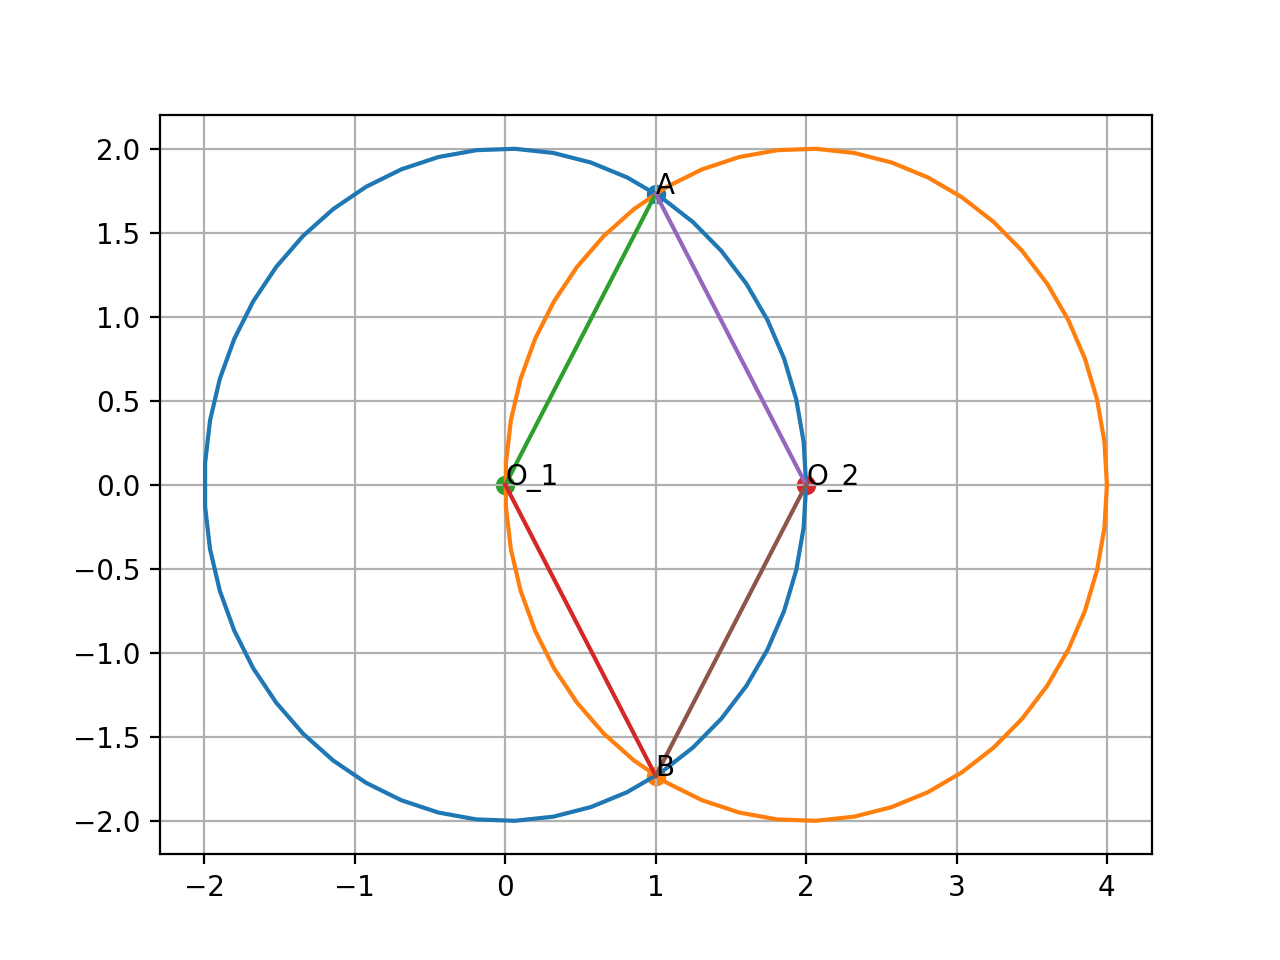
\includegraphics[width=\columnwidth]{Assignment_5.png}
	\caption{Figure depicting intersection points of circle}
	\label{myfig}
\end{figure}
 \end{document}
